% Saberes básicos (LOMLOE) asociados a esta unidad
%
% Bloque B. La materia
%   - Experimentos relacionados con los sistemas materiales: conocimiento y descripción de sus
%     propiedades, su composición y su clasificación. Técnicas de separación de mezclas.
%     Justificación: la unidad dedica una sección completa a los métodos de separación de
%     mezclas heterogéneas y homogéneas (tamizado, filtración, decantación, centrifugación,
%     extracción con disolvente, separación magnética, evaporación/cristalización, destilación
%     y cromatografía), con ejemplos y aplicaciones cotidianas (desalinización, depuradoras...).
%
% Bloque E. El cambio
%   - Los sistemas materiales: análisis de los diferentes tipos de cambios que experimentan,
%     relacionando las causas que los producen con las consecuencias que tienen.
%     Justificación: se distingue de forma explícita entre cambios físicos y químicos, con
%     ejemplos, criterios y evidencias observables para reconocerlos.
%
%   (Las reacciones químicas, la conservación de la masa y los factores que afectan a las
%    reacciones están en la Unidad 6, Las reacciones químicas.)
%
% (Traducción al español de Unit_5_Change_of_Matter.tex.)

\spacing{1.3}
\raggedbottom % pages with large figures end where the text ends (no stretched gaps between boxes)

\section{Cambios físicos y cambios químicos}

\subsection{Cambios físicos}

\begin{definition}[Cambio físico]
    Es un cambio en el que \textbf{no aparecen sustancias nuevas}: la sustancia tiene la misma fórmula química antes y después.
\end{definition}

\begin{figure}[H]
    \centering
    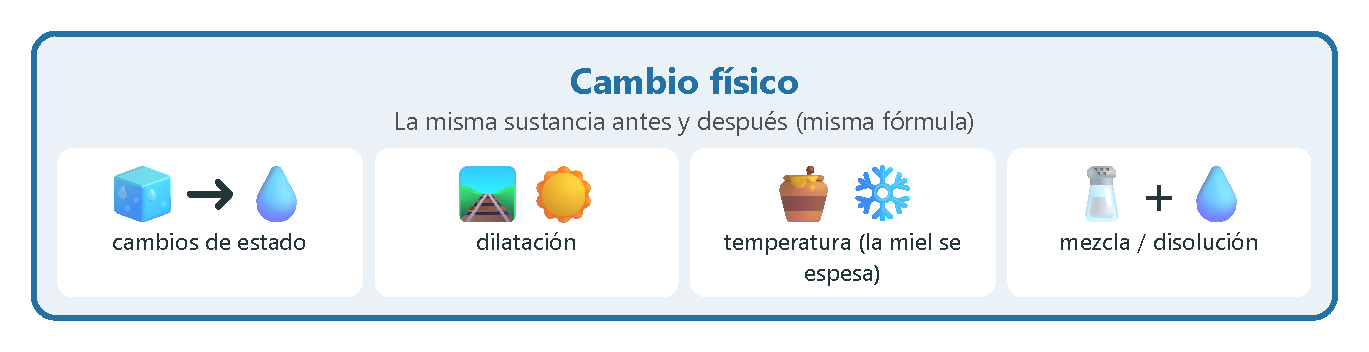
\includegraphics[width=0.85\textwidth]{FigurasSVG/Unit_5_Change_of_Matter/pdf/physical_change_es.pdf}
    \caption{Ejemplos de cambios físicos: la sustancia es la misma antes y después.}
    \label{fig:u5_physical_change}
\end{figure}

\begin{itemize}
    \item \negsubro{Cambios de temperatura}: la miel fluye mejor cuando está caliente, pero sigue siendo miel.
    \item \negsubro{Cambios de estado}: el hielo, el agua líquida y el vapor de agua son todos \ch{H2O}.
    \item \negsubro{Dilatación y contracción}: un metal se dilata al calentarlo, pero sigue siendo el mismo metal.
    \item \negsubro{Mezclas}: el hierro y el azufre en polvo mezclados siguen siendo hierro y azufre; con un imán podemos separarlos de nuevo.
\end{itemize}

\begin{exercise}
    Clasifica cada cambio físico según los cuatro tipos anteriores (cambio de temperatura, cambio de estado, dilatación/contracción, mezcla): una vía de tren en un día caluroso; congelar agua para hacer cubitos; mezclar harina y azúcar; la miel que se espesa en invierno.
    \begin{solu}
        Vía de tren: \textbf{dilatación}. \\
        Cubitos de hielo: \textbf{cambio de estado}. \\
        Harina y azúcar: \textbf{mezcla}. \\
        Miel en invierno: \textbf{cambio de temperatura} (se vuelve más viscosa).
    \end{solu}
\end{exercise}

\begin{exercise}
    Explica por qué disolver sal en agua es un cambio físico, aunque parezca que la sal desaparece.
    \begin{solu}
        No se forma ninguna sustancia nueva: la sal sigue siendo \ch{NaCl} y el agua sigue siendo \ch{H2O}, solo que mezcladas. Podemos recuperar la sal sin cambios simplemente evaporando el agua.
    \end{solu}
\end{exercise}

\subsection{Cambios químicos}

\begin{definition}[Cambio químico]
    Es un cambio en el que aparecen \textbf{sustancias nuevas}, con una fórmula distinta y propiedades diferentes.
\end{definition}

\begin{figure}[H]
    \centering
    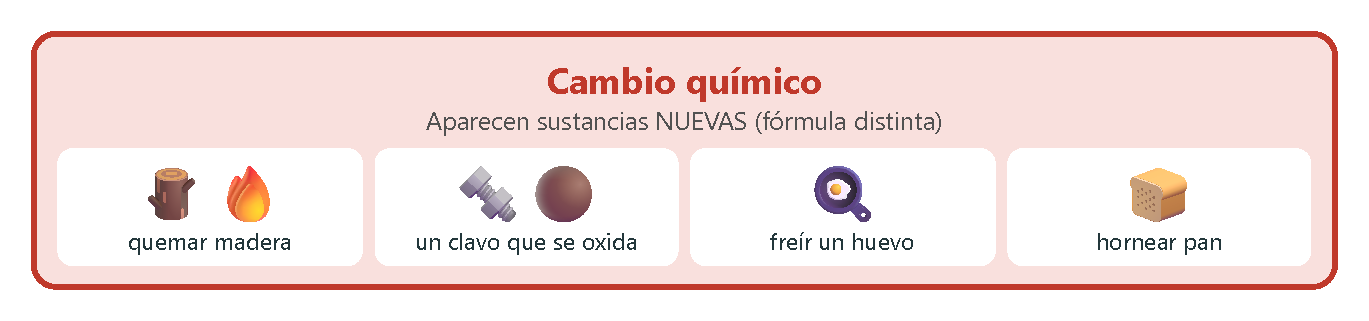
\includegraphics[width=0.85\textwidth]{FigurasSVG/Unit_5_Change_of_Matter/pdf/chemical_change_es.pdf}
    \caption{Ejemplos de cambios químicos: aparecen sustancias nuevas.}
    \label{fig:u5_chemical_change}
\end{figure}

\begin{itemize}
    \item \negsubro{Combustión}: cuando arde la madera, el papel o el gas de una cocina, reacciona con el oxígeno del aire y se transforma en sustancias nuevas, como dióxido de carbono, vapor de agua y ceniza.
    \item \negsubro{Oxidación}: un clavo que se deja a la intemperie reacciona poco a poco con el oxígeno y el agua y se cubre de óxido, una sustancia marrón que ya no es hierro.
    \item \negsubro{Cocinar alimentos}: al freír un huevo o al hornear pan se forman sustancias nuevas con otro color, sabor y textura; no podemos recuperar el huevo crudo.
    \item \negsubro{Descomposición}: una sustancia se rompe en otras más sencillas, por ejemplo cuando una corriente eléctrica descompone el agua en hidrógeno y oxígeno.
\end{itemize}

\begin{example}
    \begin{itemize}
        \item Al hacer pasar una corriente eléctrica por el agua (\ch{H2O}) se obtienen dos sustancias nuevas: hidrógeno (\ch{H2}) y oxígeno (\ch{O2}).
        \item Al calentar una mezcla de hierro y azufre se obtiene sulfuro de hierro (\ch{FeS}), una sustancia nueva que, a diferencia del hierro, \textbf{no} es atraída por un imán.
    \end{itemize}
\end{example}

\subsubsection*{¿Cambio físico o cambio químico?}

Para decidir si un cambio es físico o químico, nos preguntamos: \textbf{¿al final hay una sustancia nueva?} La figura~\ref{fig:u5_changes_signs} compara los dos tipos de cambio y muestra las \textbf{pistas} que nos indican que se está produciendo un cambio químico.

\begin{figure}[H]
    \centering
    % [FIGURA ORIGINAL] \includegraphics[width=\textwidth]{Unit_5/changes_signs}
    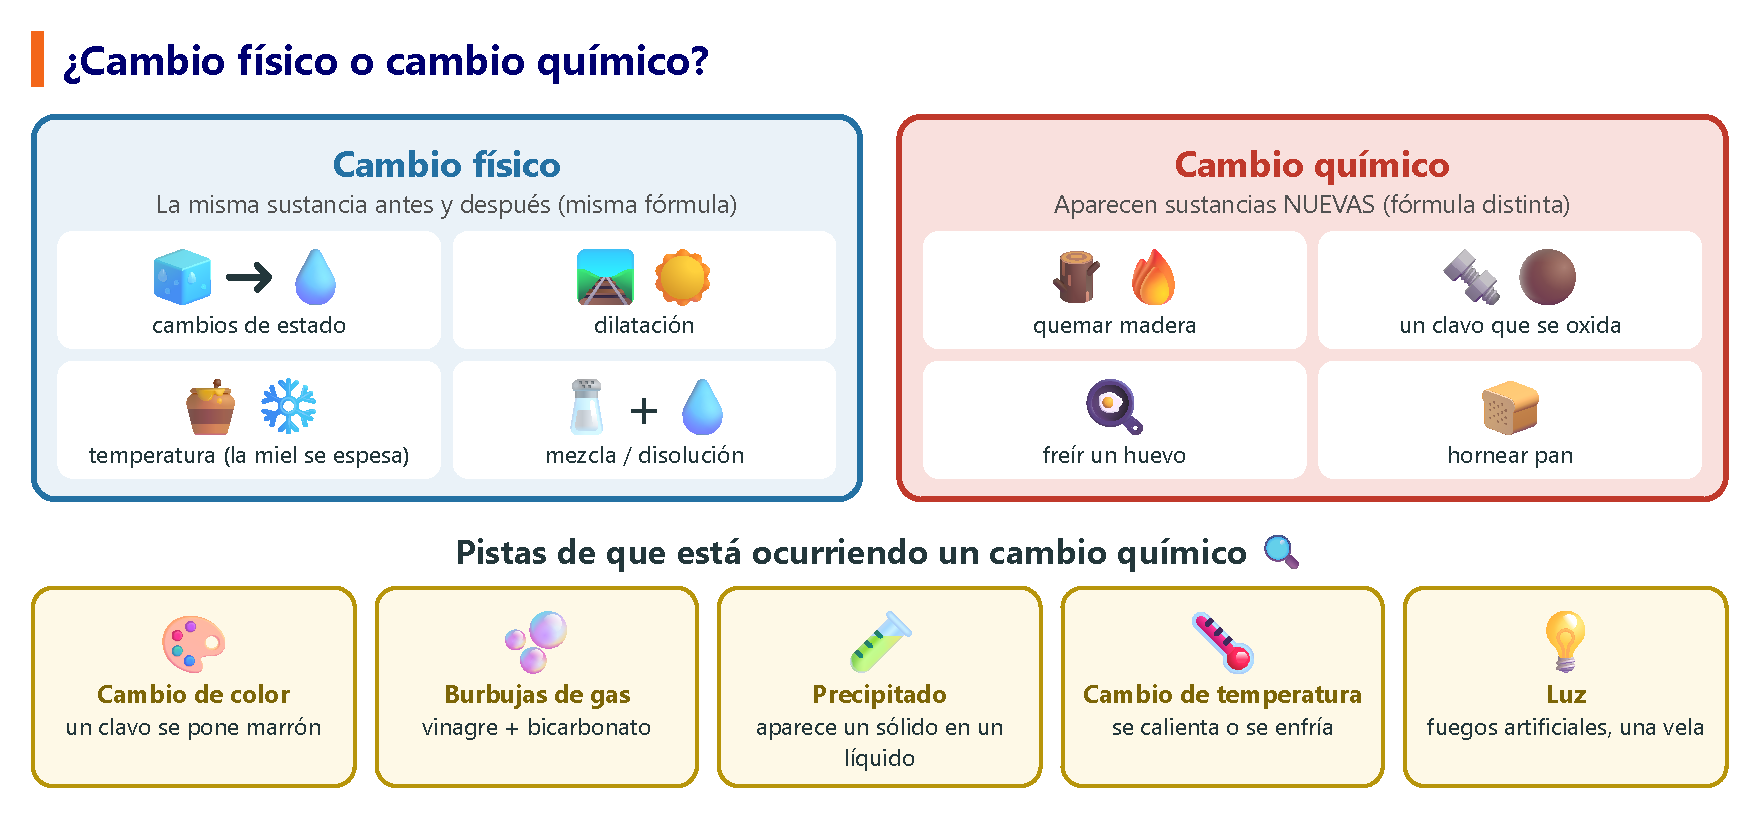
\includegraphics[width=\textwidth]{FigurasSVG/Unit_5_Change_of_Matter/pdf/changes_signs_es.pdf}
    \caption{Ejemplos de cambios físicos y químicos, y pistas que nos indican que se está produciendo un cambio químico.}
    \label{fig:u5_changes_signs}
\end{figure}

\begin{impt}
    Las pistas de la figura hacen pensar en un cambio químico, pero la única prueba \textbf{segura} es que hayan aparecido sustancias nuevas, con propiedades diferentes.
\end{impt}

\begin{exercise}
    Clasifica cada transformación como cambio \textbf{físico} o \textbf{químico}: cortar leña; encender una vela; quemar madera; batir un huevo; una llave que se oxida; el alcohol que se evapora; modelar arcilla; freír un huevo; filtrar agua con arena; hacer mayonesa; el yodo que sublima.
    \begin{solu}
        \textbf{Físicos}: cortar leña, batir un huevo, el alcohol que se evapora, modelar arcilla, filtrar agua, hacer mayonesa, el yodo que sublima. \\
        \textbf{Químicos}: encender una vela, quemar madera, una llave que se oxida, freír un huevo.
    \end{solu}
\end{exercise}

\begin{exercise}
    El aluminio se obtiene de la bauxita haciendo pasar una corriente eléctrica por el mineral fundido, y después se puede fundir y reutilizar muchas veces. ¿Estos dos procesos son cambios físicos o químicos?
    \begin{solu}
        Obtener aluminio de la bauxita: \textbf{químico} (el óxido de aluminio se transforma en aluminio metálico, una sustancia nueva). \\
        Fundir el aluminio para reutilizarlo: \textbf{físico} (solo es un cambio de estado); por eso el aluminio se puede reciclar una y otra vez.
    \end{solu}
\end{exercise}

\begin{exercise}
    ¿Cada observación corresponde más probablemente a un cambio \textbf{físico} o \textbf{químico}? Los cubitos de hielo se agrietan en una bebida templada; salen burbujas al echar vinagre sobre bicarbonato; un clavo se vuelve poco a poco de color marrón anaranjado a la intemperie; el azúcar se disuelve en el té; un fuego artificial estalla con colores brillantes.
    \begin{solu}
        Hielo que se agrieta: \textbf{físico}. \\
        Vinagre y bicarbonato: \textbf{químico} (se produce un gas, \ch{CO2}). \\
        Clavo oxidado: \textbf{químico} (cambio de color, sustancia nueva). \\
        Azúcar que se disuelve: \textbf{físico}. \\
        Fuego artificial: \textbf{químico} (luz, calor y sustancias nuevas).
    \end{solu}
\end{exercise}

\begin{exercise}
    Al mezclar una disolución de nitrato de plata con una disolución de cloruro de sodio aparece un sólido blanco que se deposita poco a poco en el fondo del tubo de ensayo. ¿Qué tipo de cambio es y qué pista te lo indica?
    \begin{solu}
        Es un \textbf{cambio químico}. La pista es la formación de un \textbf{precipitado} (un sólido insoluble que aparece dentro de un líquido).
    \end{solu}
\end{exercise}

%----------------------------------------------------------------------------------------

\section{Separación de los componentes de una mezcla}

Las sustancias de una mezcla conservan sus propiedades, así que podemos separarlas mediante \textbf{métodos físicos}, que no las transforman. Elegimos el método según la \textbf{propiedad} en la que se diferencian los componentes (tamaño, densidad, magnetismo, solubilidad, temperatura de ebullición\ldots).

\subsection{Separación de mezclas heterogéneas}

\begin{figure}[H]
    \centering
    % [FIGURA ORIGINAL] \includegraphics[width=\textwidth]{Unit_5/separation_hetero}
    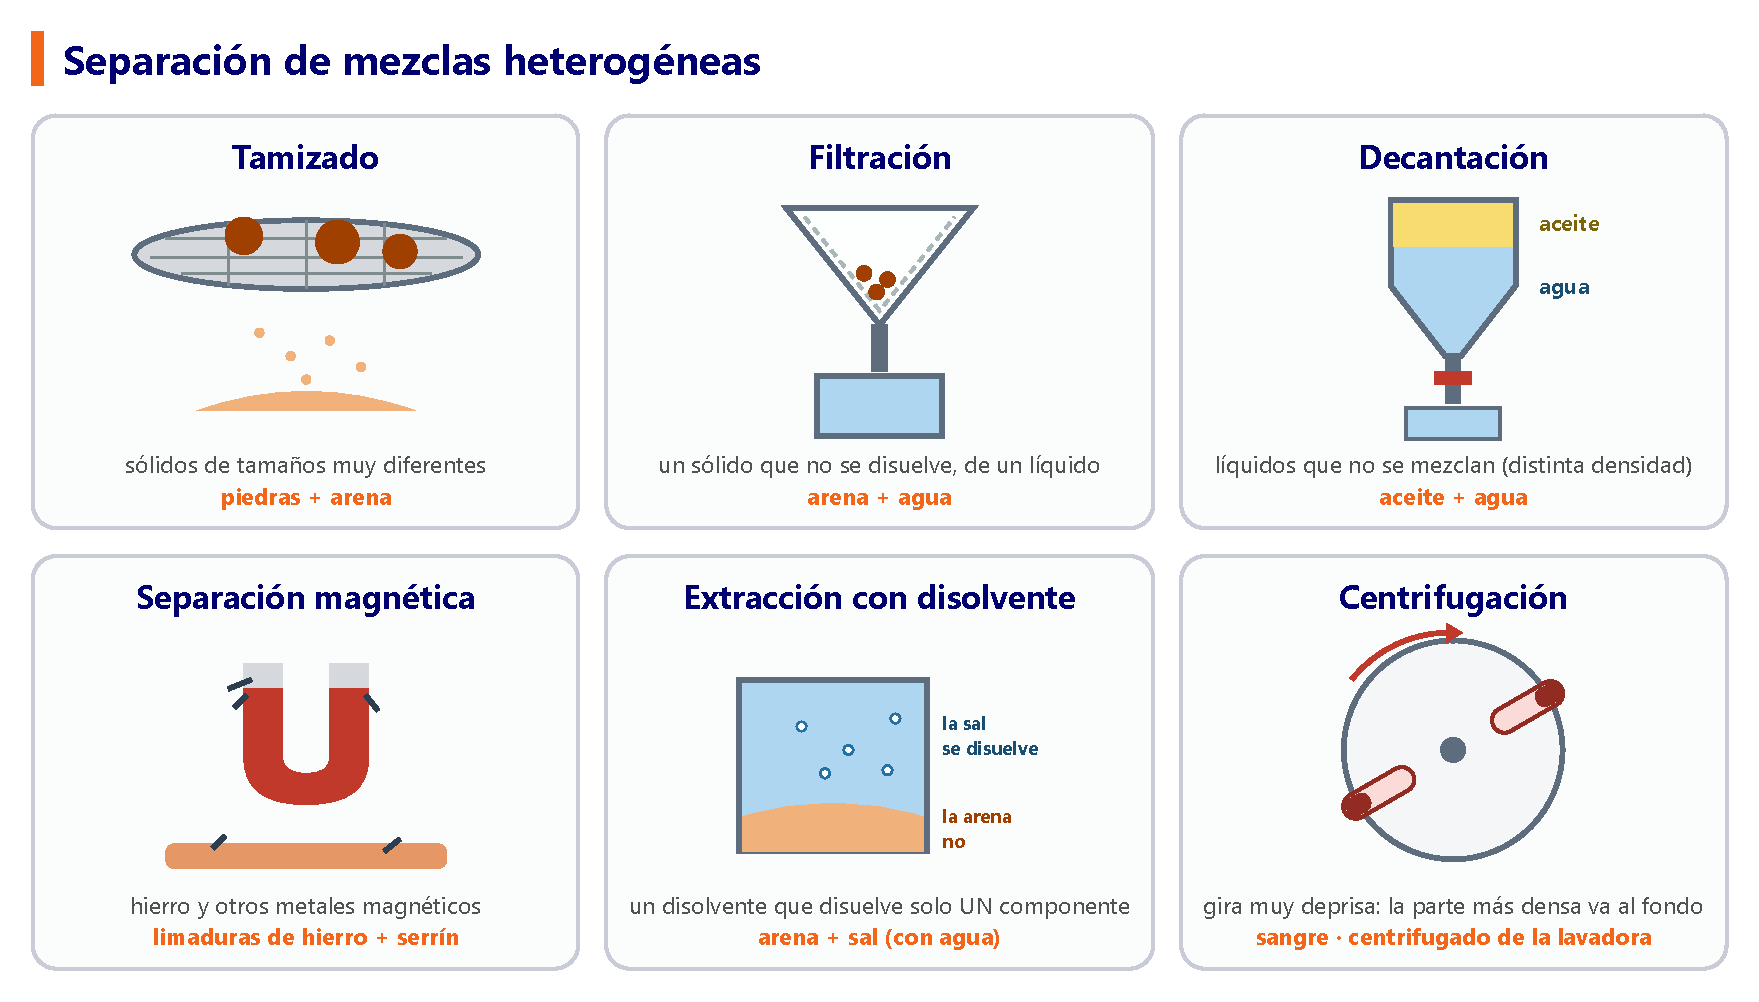
\includegraphics[width=\textwidth]{FigurasSVG/Unit_5_Change_of_Matter/pdf/separation_hetero_es.pdf}
    \caption{Métodos para separar mezclas heterogéneas.}
    \label{fig:u5_separation_hetero}
\end{figure}

\begin{figure}[H]
    \centering
    % [FIGURA ORIGINAL] \includegraphics[width=0.95\textwidth]{Unit_5/filtration}
    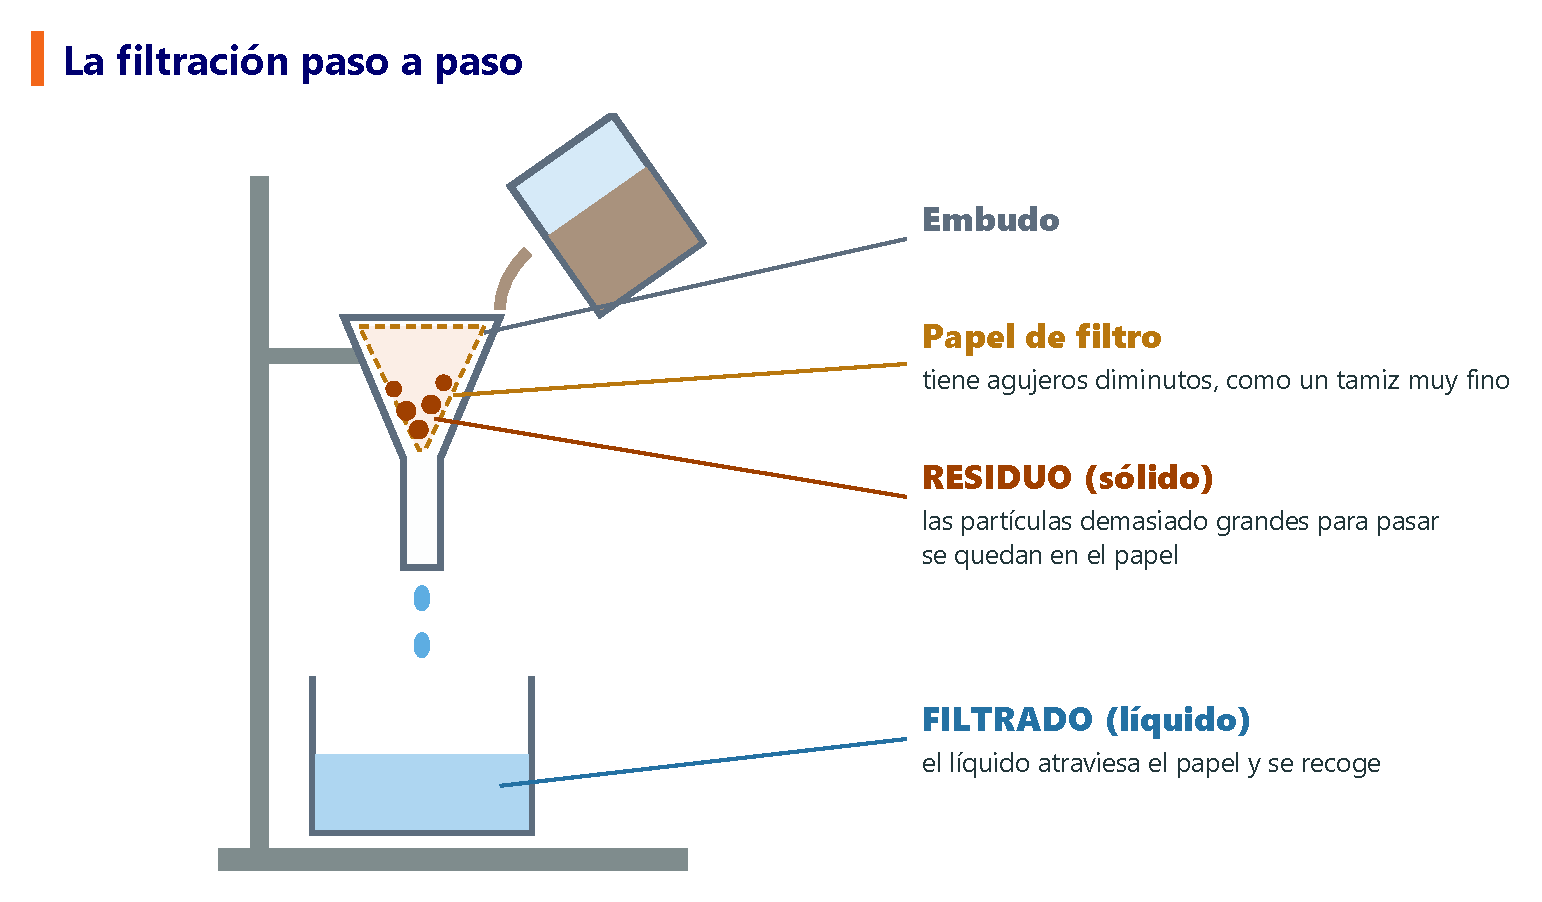
\includegraphics[width=0.95\textwidth]{FigurasSVG/Unit_5_Change_of_Matter/pdf/filtration_es.pdf}
    \caption{Filtración: el \textit{residuo} se queda en el papel y el \textit{filtrado} se recoge debajo.}
    \label{fig:u5_filtration}
\end{figure}

Veamos ahora, \textbf{paso a paso}, cómo se realiza en el laboratorio cada uno de los demás métodos.

\begin{figure}[H]
    \centering
    % [FIGURA ORIGINAL] \includegraphics[width=\textwidth]{Unit_5/sieving_steps}
    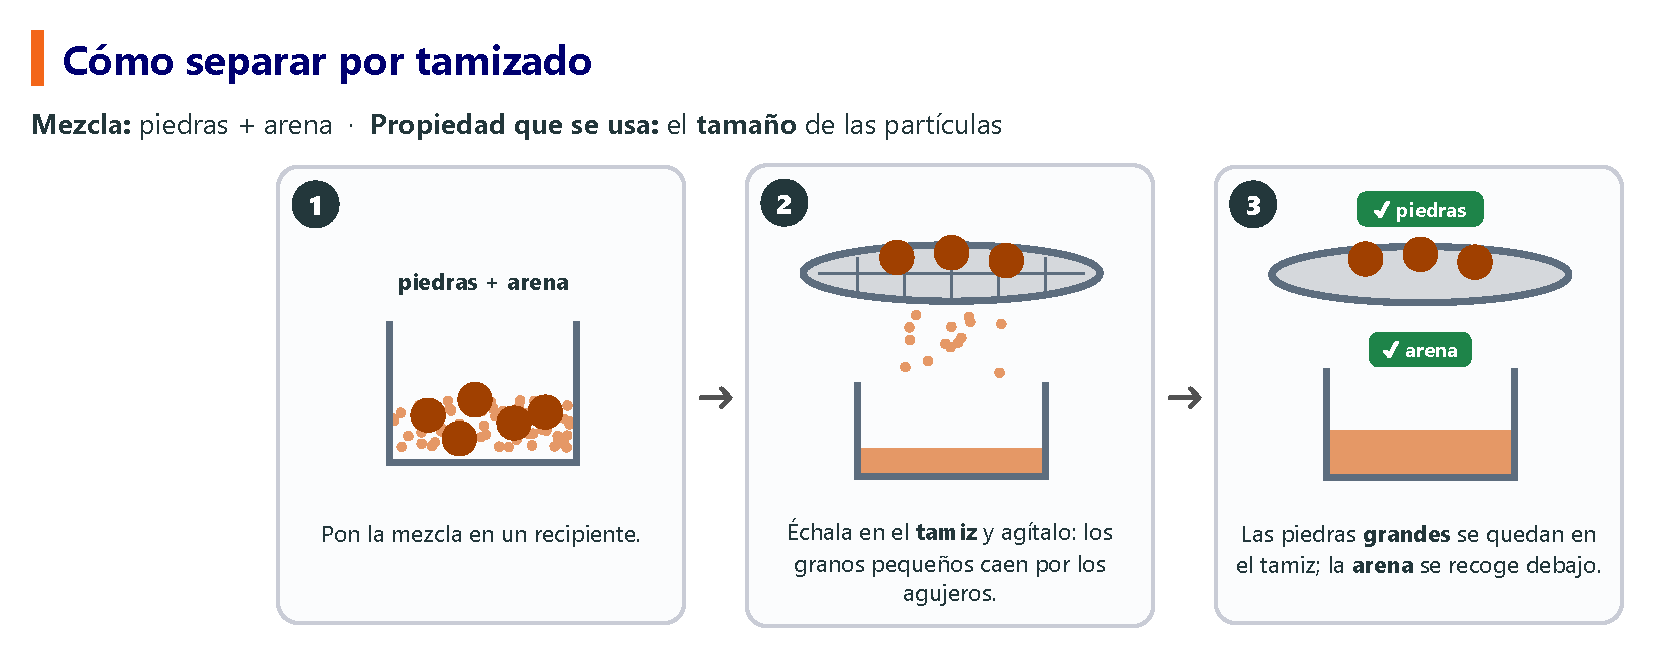
\includegraphics[width=\textwidth]{FigurasSVG/Unit_5_Change_of_Matter/pdf/sieving_steps_es.pdf}
    \caption{El tamizado paso a paso.}
    \label{fig:u5_sieving_steps}
\end{figure}

\begin{figure}[H]
    \centering
    % [FIGURA ORIGINAL] \includegraphics[width=\textwidth]{Unit_5/decantation_steps}
    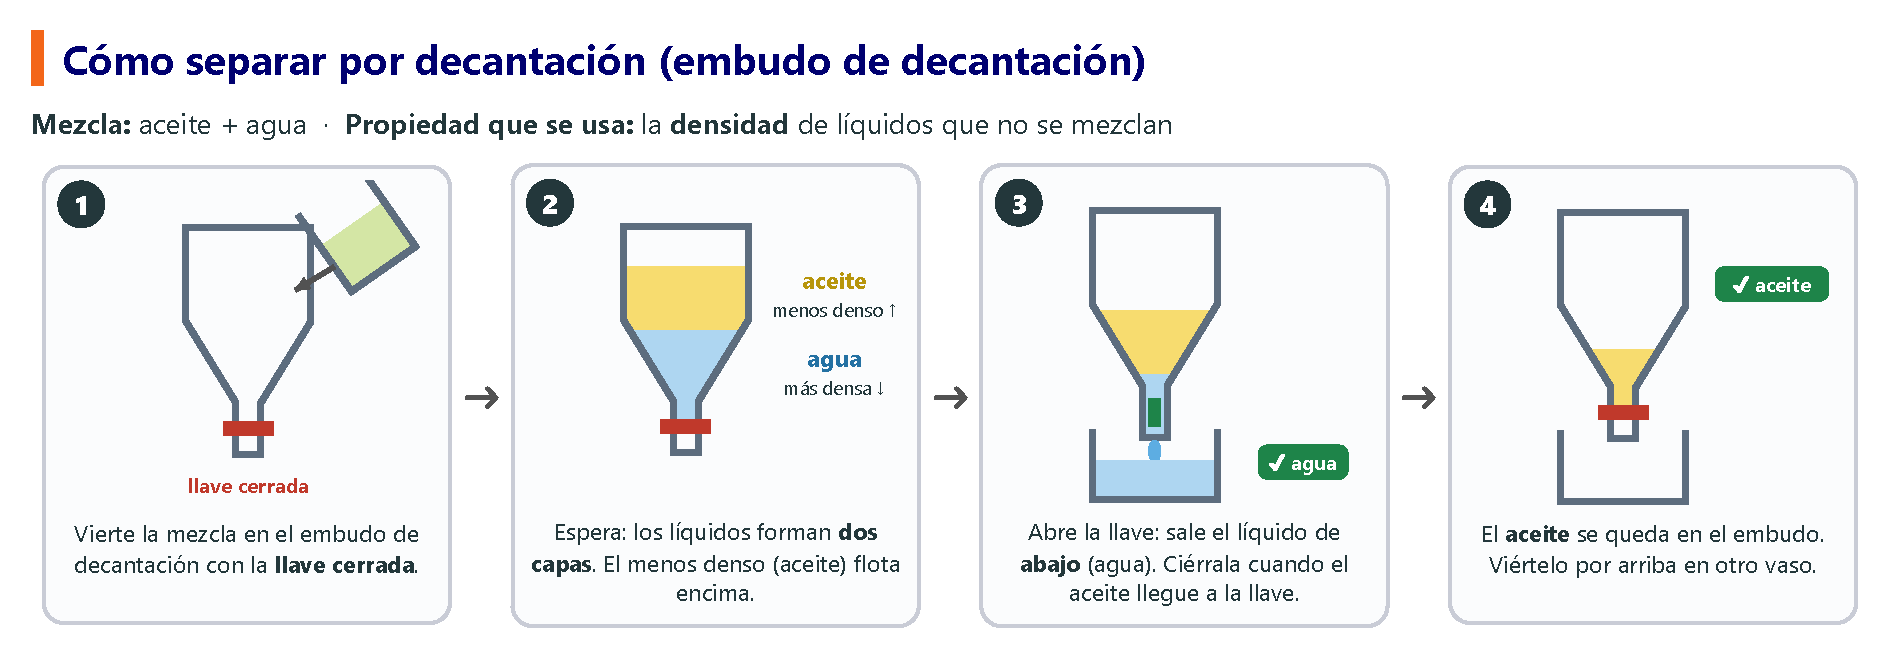
\includegraphics[width=\textwidth]{FigurasSVG/Unit_5_Change_of_Matter/pdf/decantation_steps_es.pdf}
    \caption{La decantación con embudo de decantación, paso a paso.}
    \label{fig:u5_decantation_steps}
\end{figure}

\begin{figure}[H]
    \centering
    % [FIGURA ORIGINAL] \includegraphics[width=\textwidth]{Unit_5/magnetic_steps}
    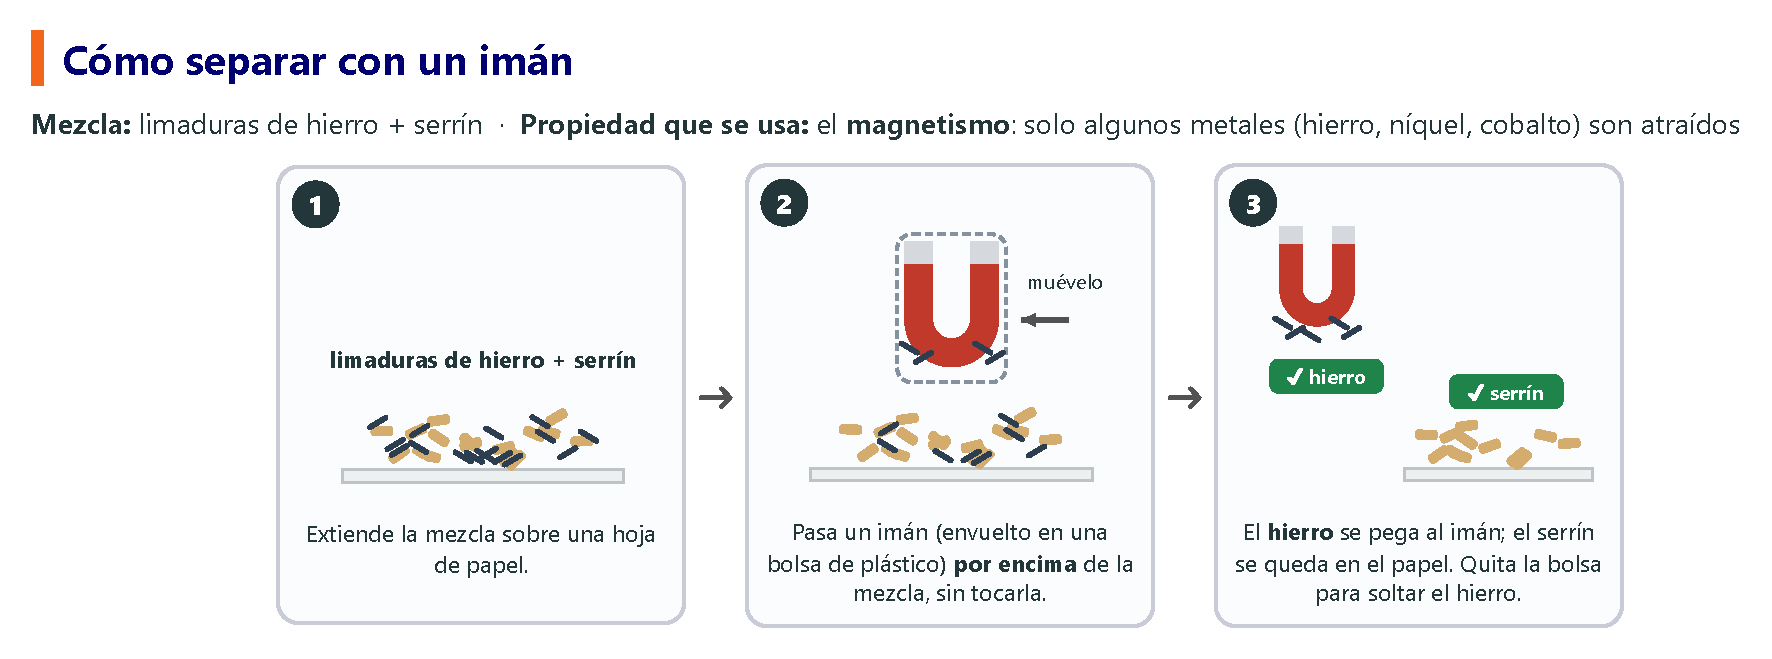
\includegraphics[width=\textwidth]{FigurasSVG/Unit_5_Change_of_Matter/pdf/magnetic_steps_es.pdf}
    \caption{La separación magnética paso a paso.}
    \label{fig:u5_magnetic_steps}
\end{figure}

\begin{figure}[H]
    \centering
    % [FIGURA ORIGINAL] \includegraphics[width=\textwidth]{Unit_5/extraction_steps}
    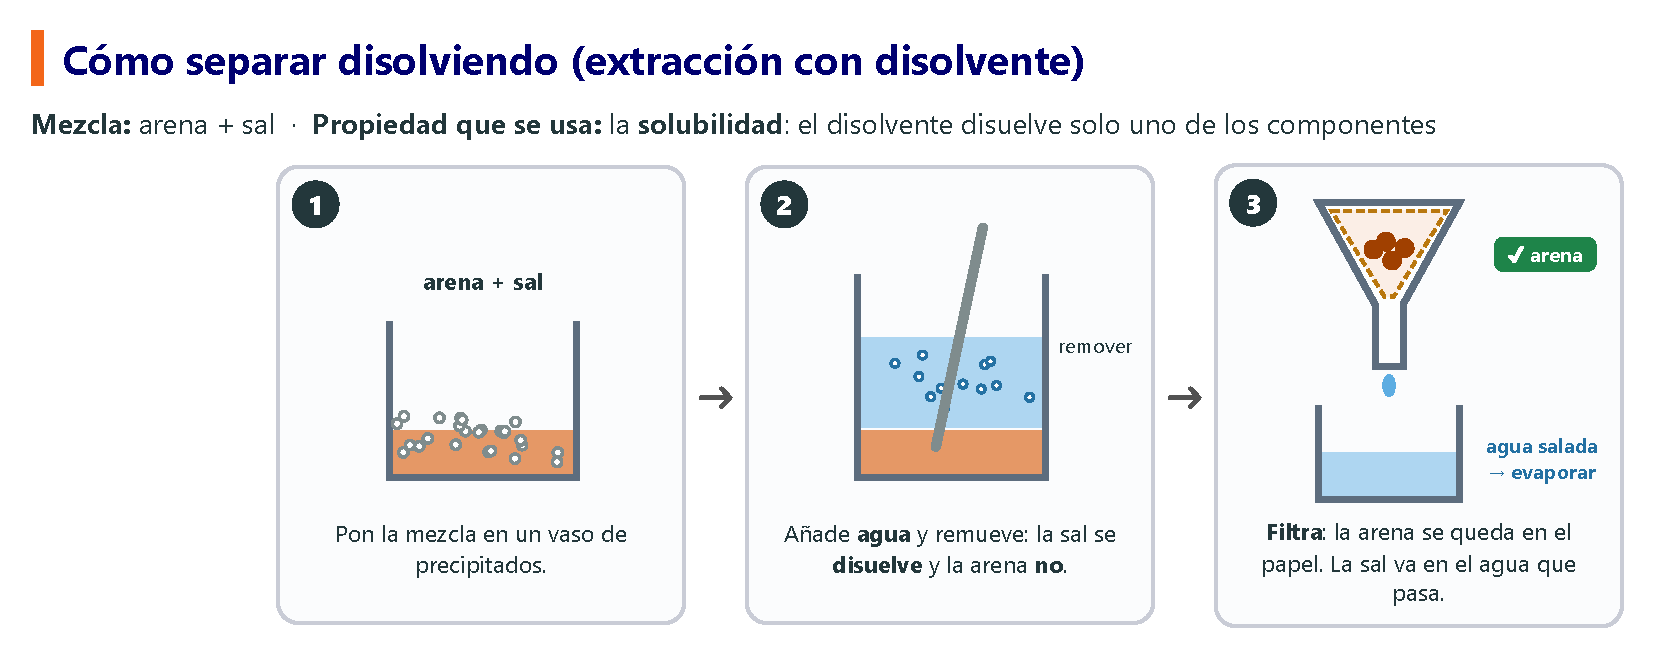
\includegraphics[width=\textwidth]{FigurasSVG/Unit_5_Change_of_Matter/pdf/extraction_steps_es.pdf}
    \caption{La extracción con disolvente (separar disolviendo) paso a paso.}
    \label{fig:u5_extraction_steps}
\end{figure}

\begin{figure}[H]
    \centering
    % [FIGURA ORIGINAL] \includegraphics[width=\textwidth]{Unit_5/centrifugation_steps}
    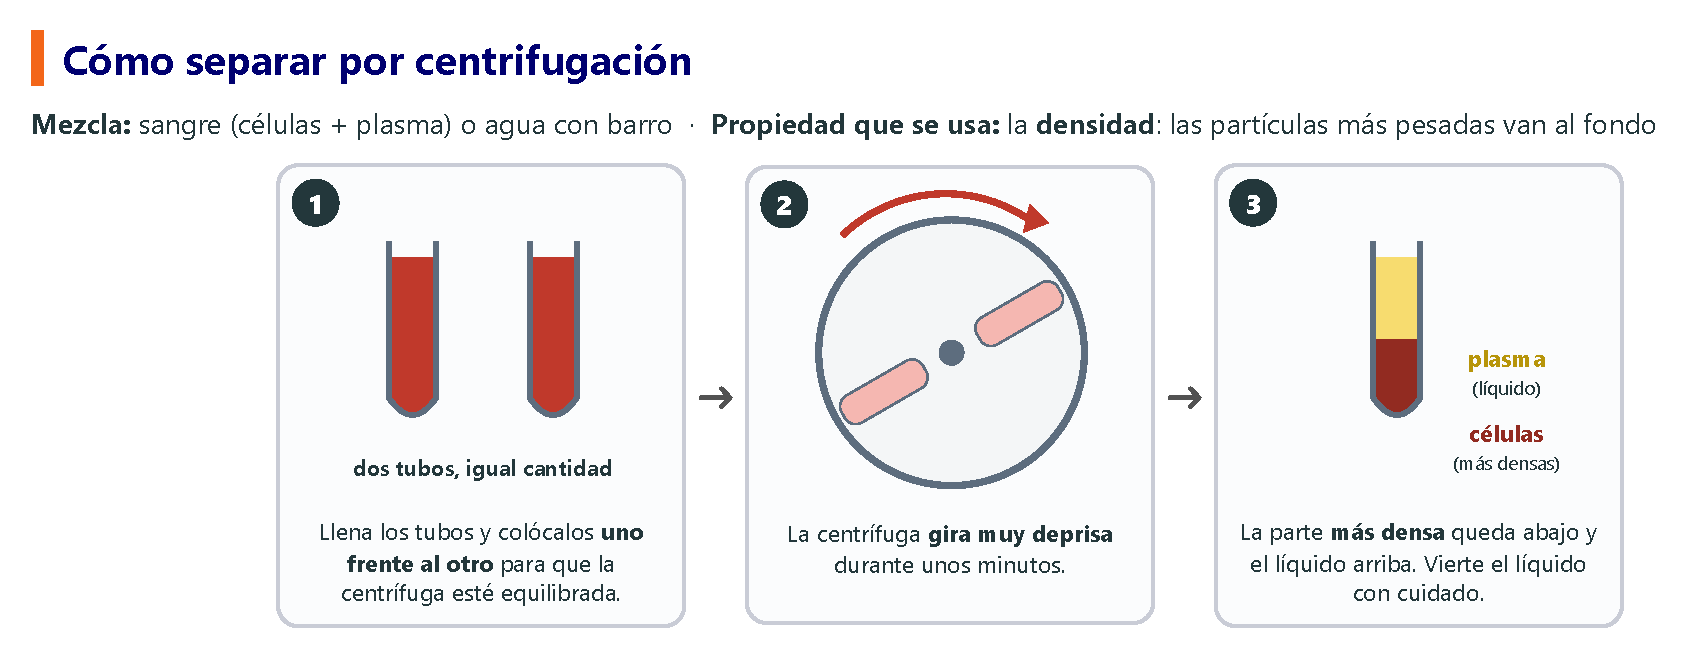
\includegraphics[width=\textwidth]{FigurasSVG/Unit_5_Change_of_Matter/pdf/centrifugation_steps_es.pdf}
    \caption{La centrifugación paso a paso.}
    \label{fig:u5_centrifugation_steps}
\end{figure}

\begin{exercise}
    Indica el mejor método de separación para cada mezcla y justifica tu elección: grava y arena fina; limaduras de hierro y virutas de madera; un aliño de ensalada hecho con vinagre y aceite de oliva.
    \begin{solu}
        Grava y arena: \textbf{tamizado} (tamaños muy distintos). \\
        Limaduras de hierro y virutas de madera: \textbf{separación magnética} (solo el hierro es atraído por un imán). \\
        Vinagre y aceite: \textbf{decantación} (líquidos que no se mezclan y tienen densidades distintas).
    \end{solu}
\end{exercise}

\begin{exercise}
    En el laboratorio del instituto se limpia una pequeña muestra de agua con barro usando un embudo y papel de filtro. En una depuradora, enormes volúmenes de agua con barro se dejan reposar varias horas en grandes tanques. Indica la técnica que se usa en cada caso y explica por qué la depuradora no utiliza papel de filtro.
    \begin{solu}
        Laboratorio: \textbf{filtración}. Depuradora: \textbf{decantación} (sedimentación). Filtrar volúmenes tan grandes con papel sería demasiado lento y los filtros se atascarían; dejar que la tierra se deposite por la gravedad es más barato y funciona bien con grandes cantidades.
    \end{solu}
\end{exercise}

\subsection{Separación de mezclas homogéneas}

\begin{figure}[H]
    \centering
    % [FIGURA ORIGINAL] \includegraphics[width=\textwidth]{Unit_5/separation_homo}
    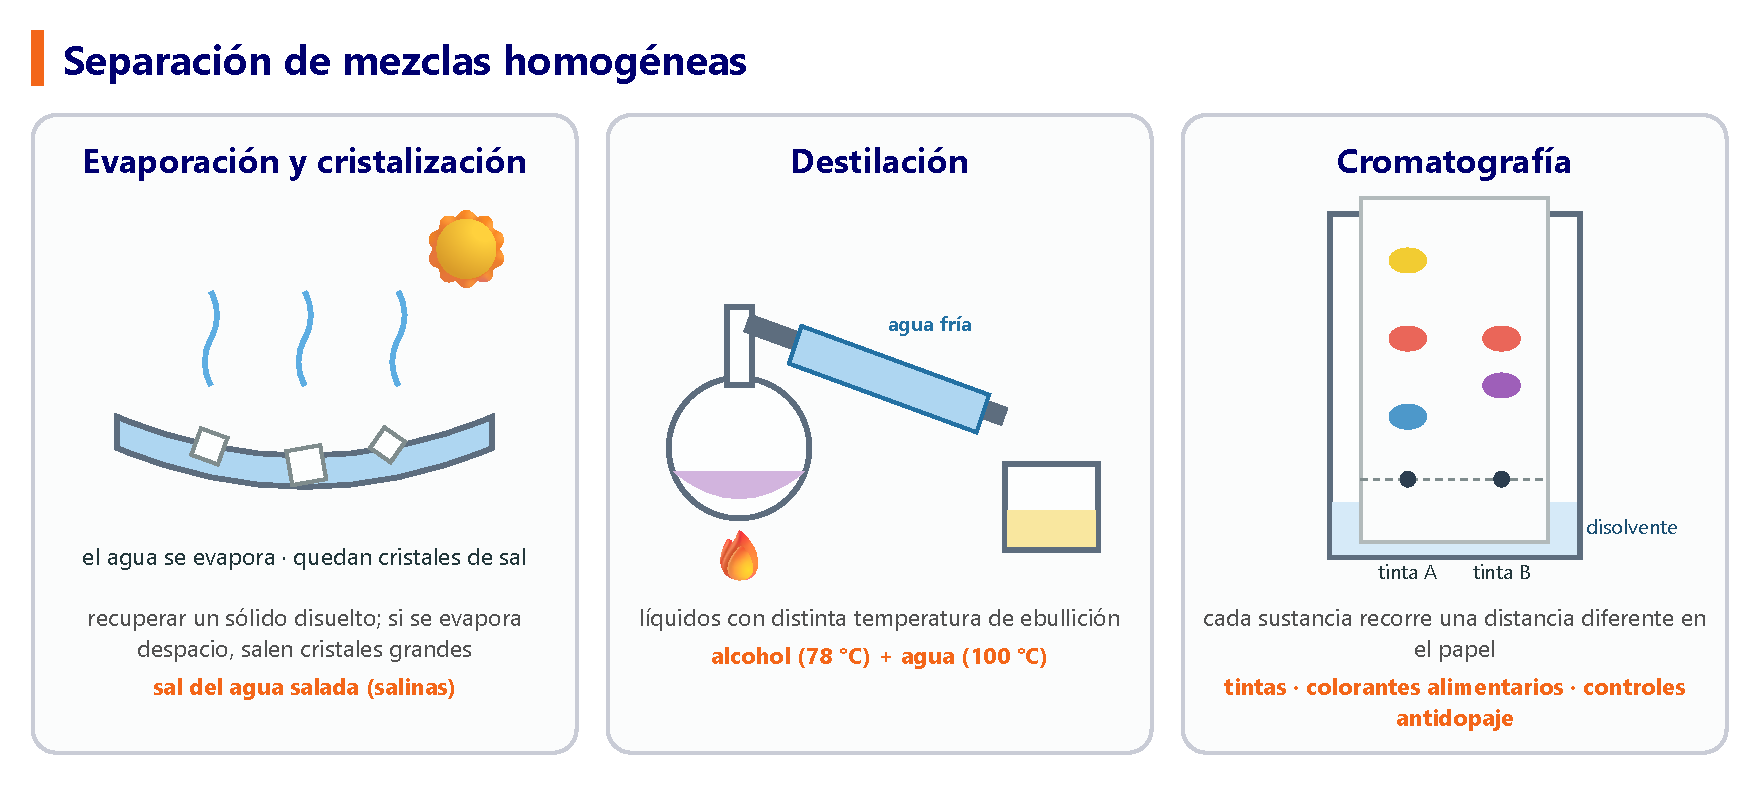
\includegraphics[width=\textwidth]{FigurasSVG/Unit_5_Change_of_Matter/pdf/separation_homo_es.pdf}
    \caption{Métodos para separar mezclas homogéneas.}
    \label{fig:u5_separation_homo}
\end{figure}

\begin{figure}[H]
    \centering
    % [FIGURA ORIGINAL] \includegraphics[width=\textwidth]{Unit_5/distillation}
    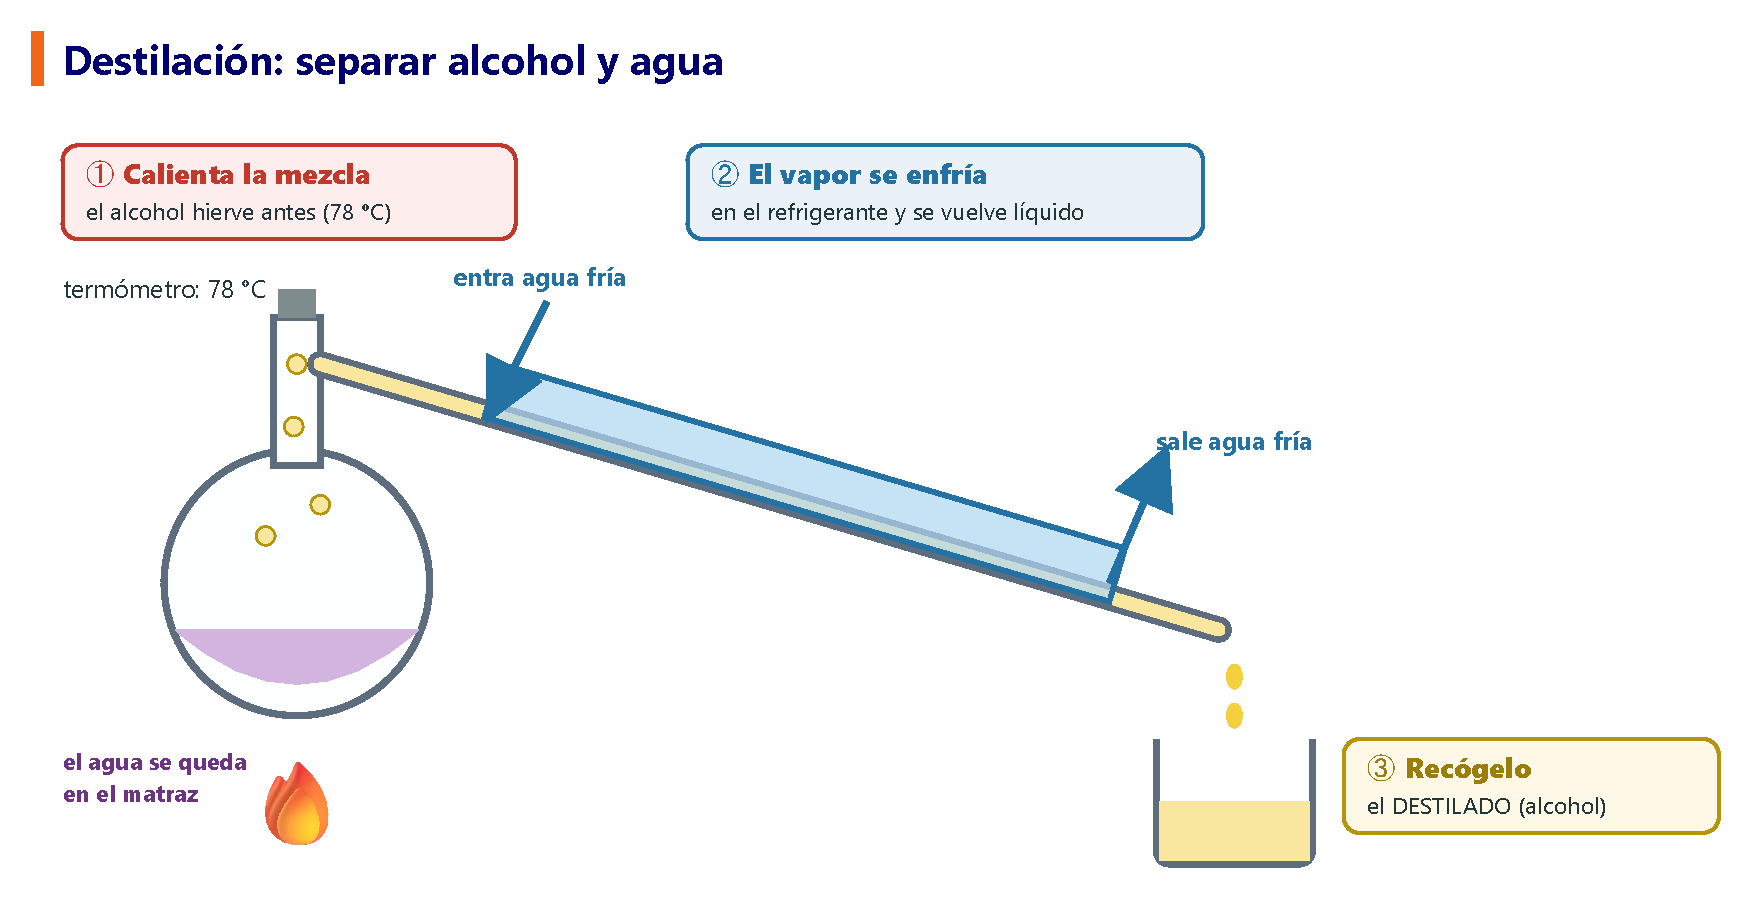
\includegraphics[width=\textwidth]{FigurasSVG/Unit_5_Change_of_Matter/pdf/distillation_es.pdf}
    \caption{Destilación: el líquido con menor temperatura de ebullición se evapora primero y se condensa en el refrigerante.}
    \label{fig:u5_distillation}
\end{figure}

\begin{figure}[H]
    \centering
    % [FIGURA ORIGINAL] \includegraphics[width=\textwidth]{Unit_5/evaporation_steps}
    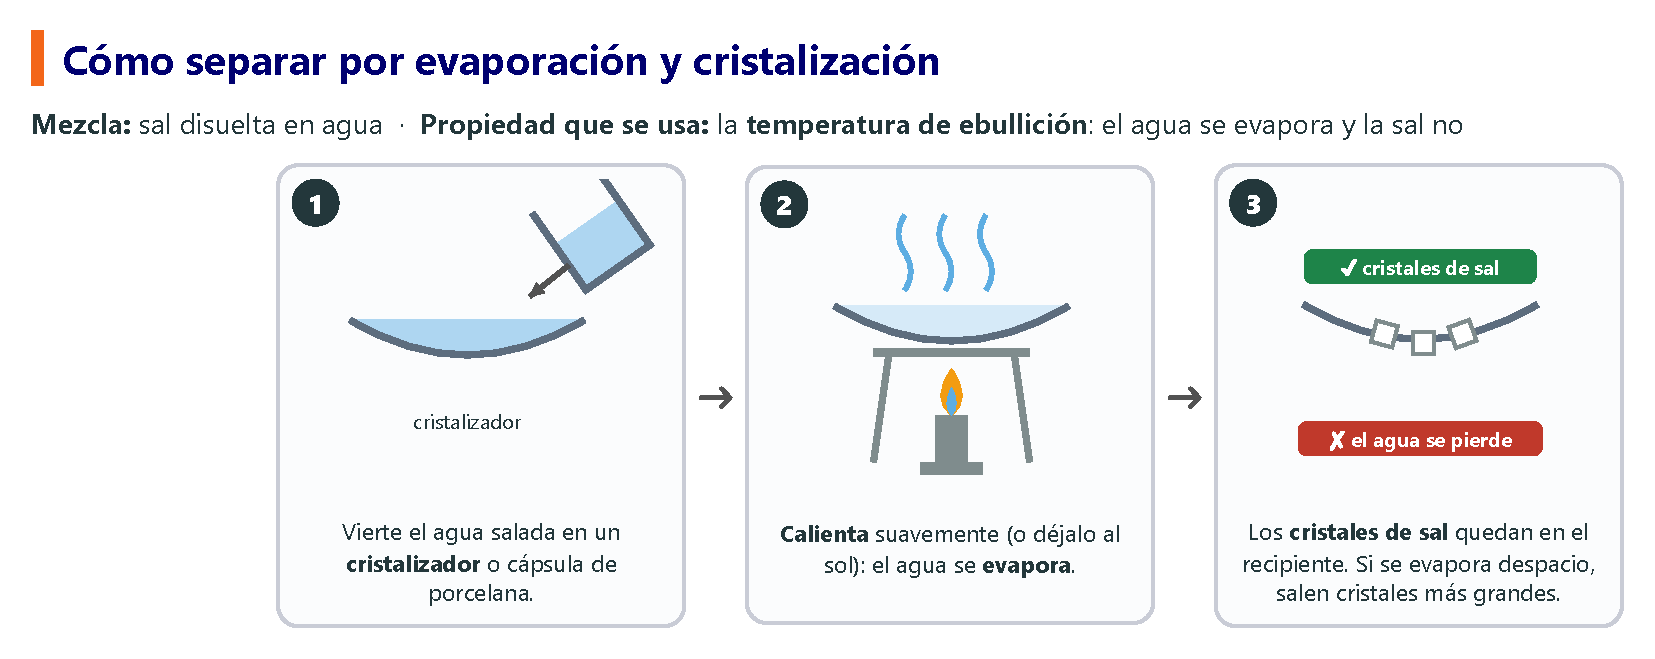
\includegraphics[width=\textwidth]{FigurasSVG/Unit_5_Change_of_Matter/pdf/evaporation_steps_es.pdf}
    \caption{La evaporación y la cristalización paso a paso.}
    \label{fig:u5_evaporation_steps}
\end{figure}

\begin{figure}[H]
    \centering
    % [FIGURA ORIGINAL] \includegraphics[width=\textwidth]{Unit_5/chromatography_steps}
    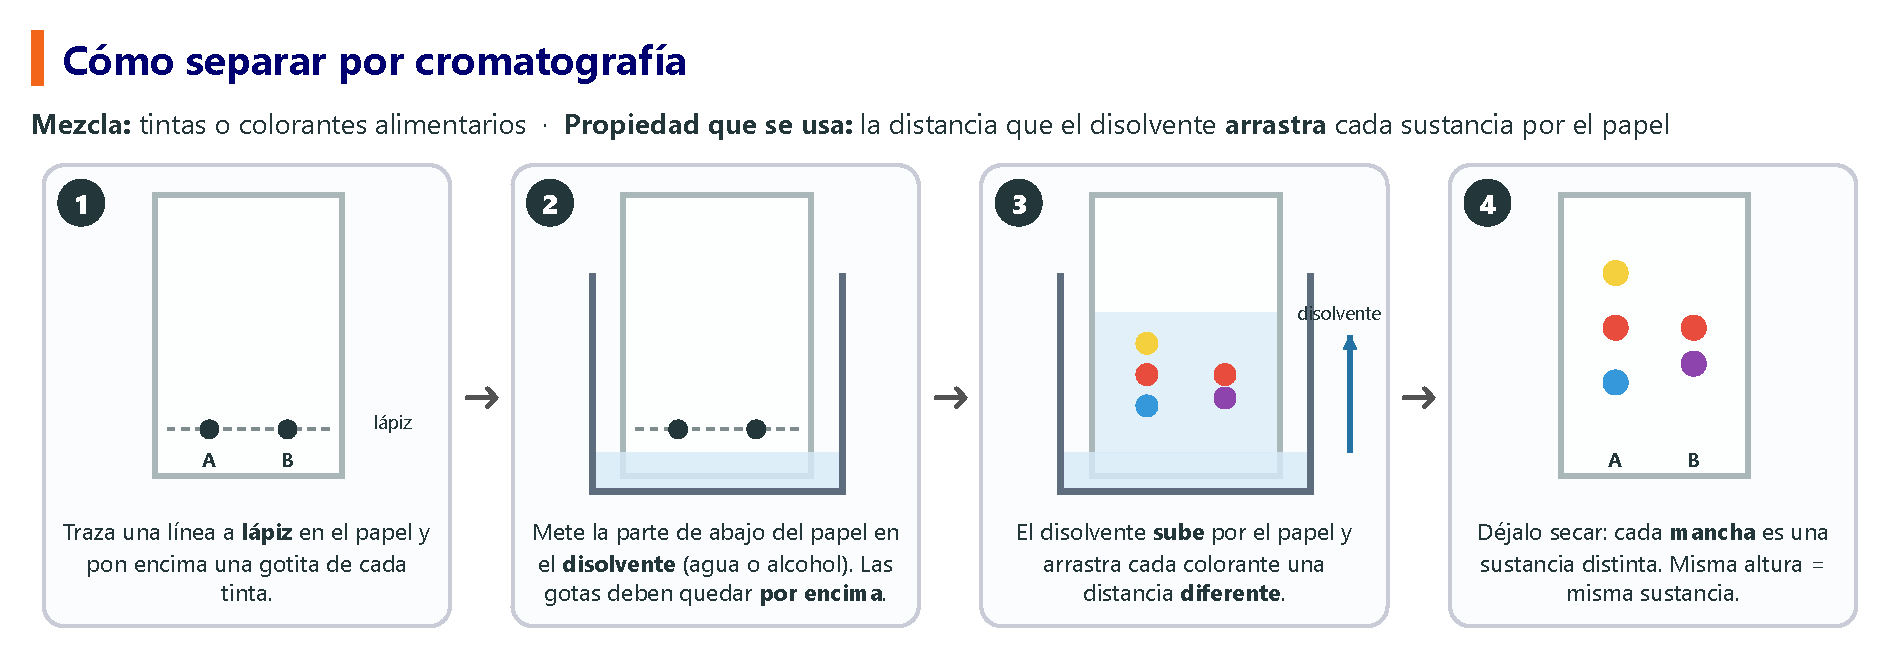
\includegraphics[width=\textwidth]{FigurasSVG/Unit_5_Change_of_Matter/pdf/chromatography_steps_es.pdf}
    \caption{La cromatografía en papel paso a paso.}
    \label{fig:u5_chromatography_steps}
\end{figure}

\begin{didyouknow}
    Muchos lugares donde llueve poco, como las islas Canarias, obtienen el agua potable del mar en \textbf{plantas desalinizadoras}. Primero se filtra el agua de mar y después se le quitan las sales por destilación o haciendo pasar el agua a presión a través de membranas especiales.
\end{didyouknow}

\begin{exercise}
    Un perfume es una mezcla homogénea de varias sustancias aromáticas disueltas en alcohol, cada una con una temperatura de ebullición distinta. ¿Qué técnica usarías para recuperar el alcohol y en qué propiedad se basa?
    \begin{solu}
        \textbf{Destilación}. Se basa en las \textbf{distintas temperaturas de ebullición}: la sustancia con la temperatura de ebullición más baja se evapora primero y se puede condensar y recoger por separado.
    \end{solu}
\end{exercise}

\begin{exercise}
    Una científica forense necesita saber si la tinta de una nota coincide con la del bolígrafo de un sospechoso. ¿Qué técnica debe usar y cómo permite comparar las dos tintas?
    \begin{solu}
        \textbf{Cromatografía}. Se pone una gota de cada tinta en papel de filtro con un disolvente; cada colorante avanza una distancia distinta y se forma un dibujo de manchas de colores. Si los dos dibujos son iguales, lo más probable es que las tintas sean la misma.
    \end{solu}
\end{exercise}

\begin{exercise}
    Ordena correctamente estos pasos de la destilación de una mezcla de alcohol y agua: el alcohol se condensa; la mezcla alcanza la temperatura de ebullición del alcohol; el alcohol se vaporiza; el alcohol líquido se recoge en otro recipiente.
    \begin{solu}
        1.\ La mezcla alcanza la temperatura de ebullición del alcohol (\qty{78}{\celsius}). \\
        2.\ El alcohol se vaporiza. \\
        3.\ El alcohol se condensa en el refrigerante. \\
        4.\ El alcohol líquido se recoge en otro recipiente.
    \end{solu}
\end{exercise}

\subsection{Varias técnicas de separación seguidas}

Las mezclas reales suelen necesitar \textbf{varios} métodos, uno detrás de otro:

\begin{figure}[H]
    \centering
    % [FIGURA ORIGINAL] \includegraphics[width=\textwidth]{Unit_5/separation_steps}
    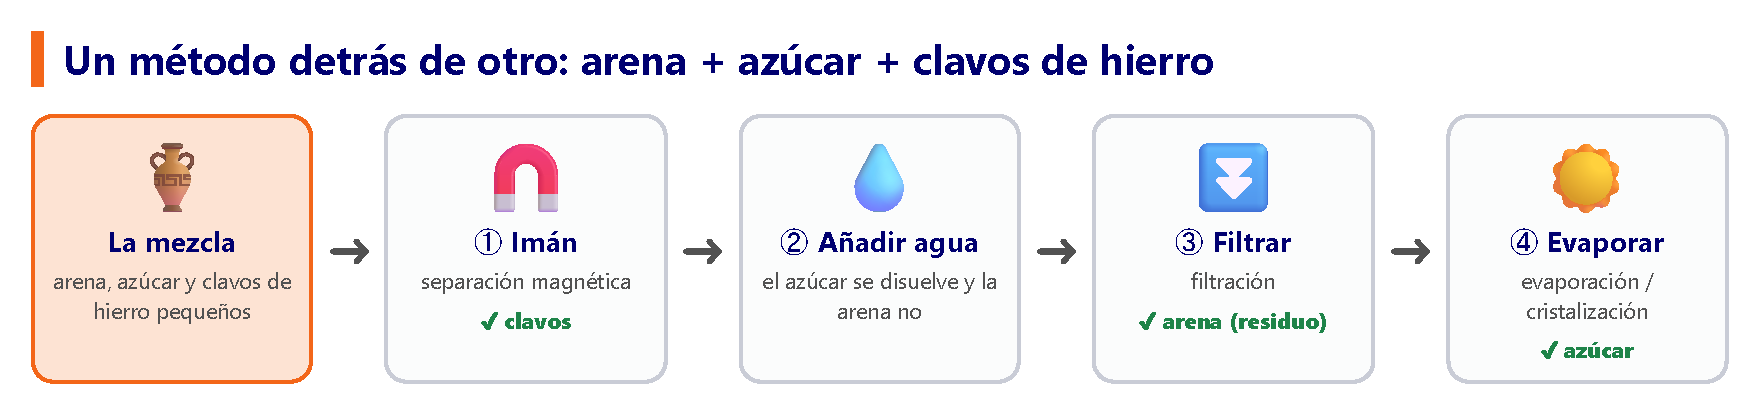
\includegraphics[width=\textwidth]{FigurasSVG/Unit_5_Change_of_Matter/pdf/separation_steps_es.pdf}
    \caption{Separación paso a paso de una mezcla de tres componentes.}
    \label{fig:u5_separation_steps}
\end{figure}

\begin{impt}
    \negsubro{¿Qué me quedo y qué tiro?} Después de cada paso la mezcla queda dividida en dos partes. Antes de empezar, lee bien el ejercicio para saber \textbf{qué quieres obtener} y, después de cada paso, decide qué haces con cada parte:
    \begin{itemize}
        \item \textcolor{green!50!black}{\textbf{ME LO QUEDO}}: es una de las sustancias que queremos obtener.
        \item \textcolor{blue!70!black}{\textbf{SIGUIENTE PASO}}: todavía es una mezcla, así que seguimos separándola.
        \item \textcolor{red!70!black}{\textbf{LO DESECHO}}: no lo necesitamos (lo tiramos o lo llevamos a un punto limpio).
    \end{itemize}
    Ten especial cuidado cuando hay un \textbf{sólido y un líquido}, como en la filtración: el sólido que se queda en el papel es el \textbf{residuo} y el líquido que pasa es el \textbf{filtrado}. Cualquiera de los dos puede ser la parte que nos quedamos, la que pasa al siguiente paso o la que desechamos: depende de lo que queramos obtener.
\end{impt}

\begin{example}
    \textbf{Ejemplo resuelto 1. Tenemos una mezcla de arena, sal y limaduras de hierro. Queremos obtener los tres componentes por separado.}
\end{example}

\begin{figure}[H]
    \centering
    % [FIGURA ORIGINAL] \includegraphics[width=\textwidth]{Unit_5/example_sand_salt_iron}
    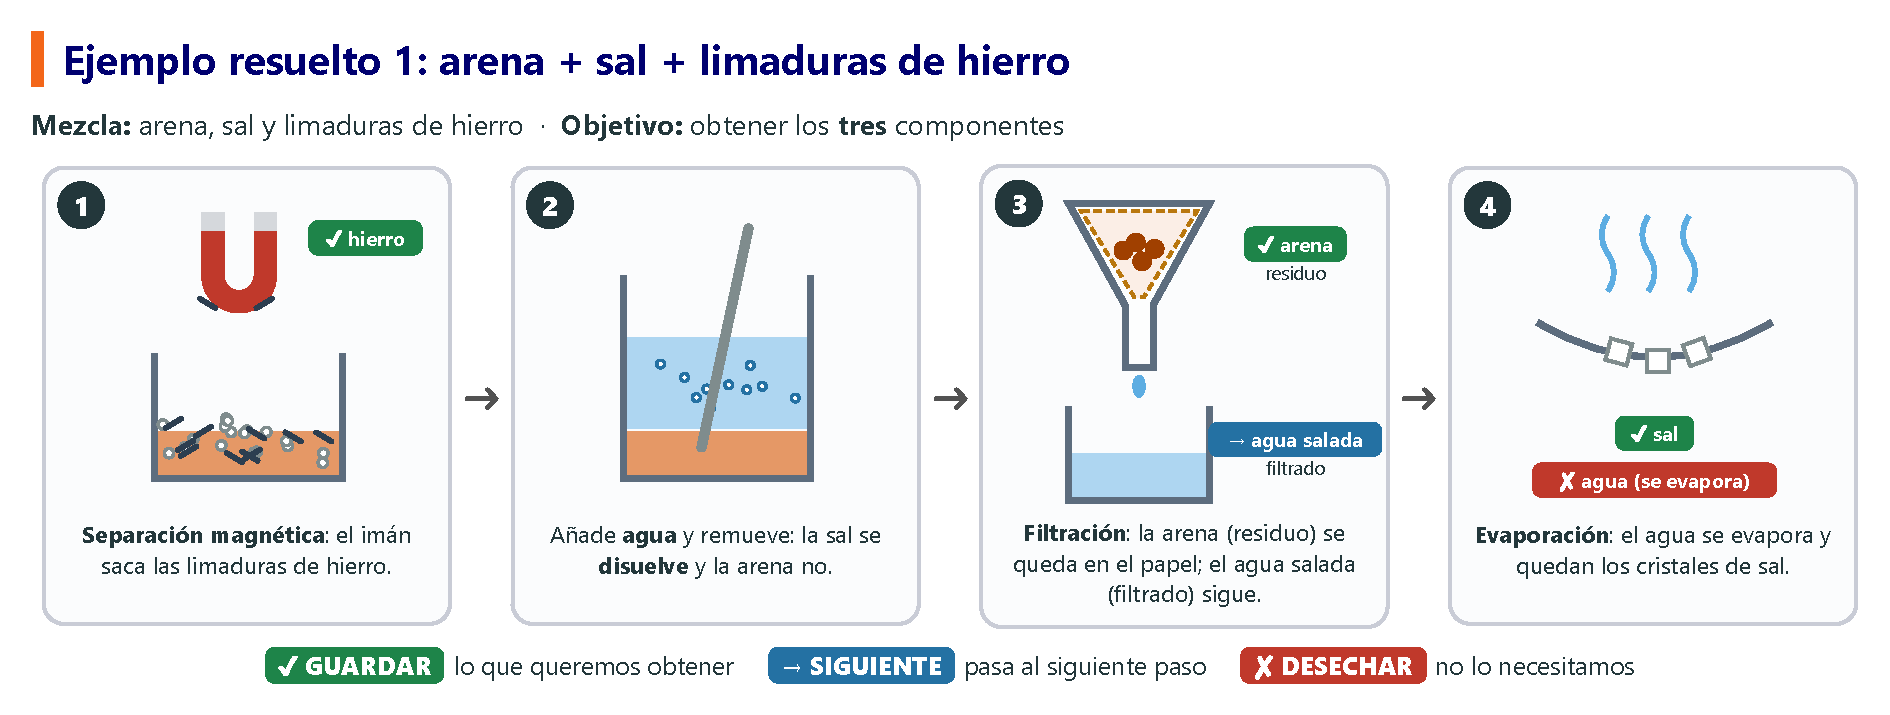
\includegraphics[width=\textwidth]{FigurasSVG/Unit_5_Change_of_Matter/pdf/example_sand_salt_iron_es.pdf}
    \caption{Ejemplo resuelto 1: separación de arena, sal y limaduras de hierro.}
    \label{fig:u5_example_sand_salt_iron}
\end{figure}

\begin{enumerate}[label=\numberballmDarkTeal]
    \item \textbf{Separación magnética.} Pasamos un imán por encima de la mezcla. Solo es atraído el hierro. \textcolor{green!50!black}{\textbf{Me lo quedo}}: las limaduras de hierro. \textcolor{blue!70!black}{\textbf{Siguiente paso}}: arena + sal.
    \item \textbf{Disolución.} Añadimos agua a la arena y la sal y removemos. La sal se disuelve; la arena no.
    \item \textbf{Filtración.} Filtramos la mezcla. \textcolor{green!50!black}{\textbf{Me lo quedo}}: la arena (\textbf{residuo}), que dejamos secar. \textcolor{blue!70!black}{\textbf{Siguiente paso}}: el agua salada (\textbf{filtrado}).
    \item \textbf{Evaporación.} Calentamos el agua salada en una cápsula de porcelana. \textcolor{green!50!black}{\textbf{Me lo quedo}}: los cristales de sal. El agua se evapora: la \textcolor{red!70!black}{\textbf{perdemos}}, pero no la necesitábamos.
\end{enumerate}

\begin{tcolorbox}[enhanced, breakable, colback=yellow!6!white, colframe=ocre, boxrule=0.8pt, arc=2mm,
    fonttitle=\sffamily\bfseries, title={Cómo escribirlo en el cuaderno}]
    \textbf{Mezcla}: arena + sal + limaduras de hierro. \quad \textbf{Objetivo}: obtener los tres componentes.

    \begin{tabular}{@{}p{0.3cm}>{\raggedright\arraybackslash}p{2.9cm}>{\raggedright\arraybackslash}p{3.9cm}>{\raggedright\arraybackslash}p{4.2cm}@{}}
        \toprule
        & \textbf{Método} & \textbf{¿Por qué? (propiedad)} & \textbf{Resultado} \\
        \midrule
        1 & Separación magnética & el hierro es atraído por los imanes & \textbf{hierro} (me lo quedo); arena + sal (siguiente) \\
        2 & Disolver en agua & la sal es soluble y la arena no & arena + agua salada (siguiente) \\
        3 & Filtración & la arena no atraviesa el papel & residuo: \textbf{arena} (me la quedo); filtrado: agua salada (siguiente) \\
        4 & Evaporación & el agua se evapora y la sal no & \textbf{sal} (me la quedo); agua (se pierde) \\
        \bottomrule
    \end{tabular}
\end{tcolorbox}

\begin{example}
    \textbf{Ejemplo resuelto 2. Un cubo contiene agua sucia con barro y aceite: arena, aceite y agua. Queremos obtener agua limpia.}
\end{example}

\begin{figure}[H]
    \centering
    % [FIGURA ORIGINAL] \includegraphics[width=\textwidth]{Unit_5/example_sand_oil_water}
    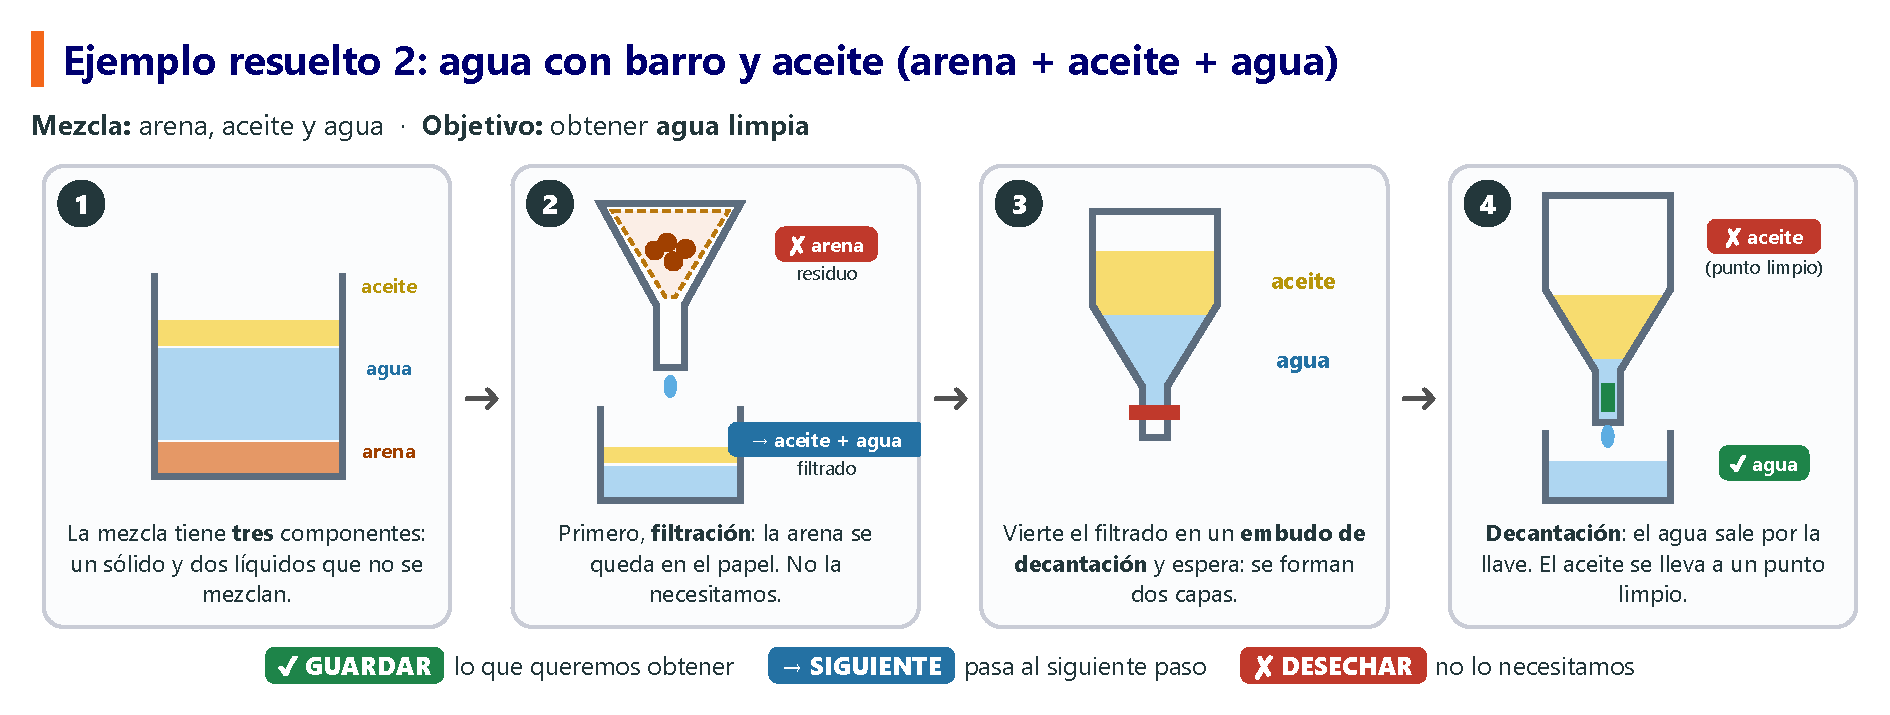
\includegraphics[width=\textwidth]{FigurasSVG/Unit_5_Change_of_Matter/pdf/example_sand_oil_water_es.pdf}
    \caption{Ejemplo resuelto 2: obtención de agua limpia a partir de una mezcla de arena, aceite y agua.}
    \label{fig:u5_example_sand_oil_water}
\end{figure}

\begin{enumerate}[label=\numberballmDarkTeal]
    \item Observamos la mezcla: un sólido (arena) y dos líquidos que no se mezclan (aceite y agua).
    \item \textbf{Primero, filtración}, para que la arena no atasque la llave del embudo de decantación. \textcolor{red!70!black}{\textbf{Lo desecho}}: la arena (\textbf{residuo}), porque solo queremos el agua. \textcolor{blue!70!black}{\textbf{Siguiente paso}}: aceite + agua (\textbf{filtrado}).
    \item Echamos el filtrado en un \textbf{embudo de decantación} y esperamos a que se formen dos capas: el aceite, menos denso, arriba; el agua, más densa, abajo.
    \item \textbf{Decantación.} Abrimos la llave y dejamos salir el agua, y la cerramos cuando el aceite llega a la llave. \textcolor{green!50!black}{\textbf{Me lo quedo}}: el agua limpia. \textcolor{red!70!black}{\textbf{Lo desecho}}: el aceite, que \textbf{nunca} debe tirarse por el fregadero: lo llevamos a un punto limpio.
\end{enumerate}

\begin{tcolorbox}[enhanced, breakable, colback=yellow!6!white, colframe=ocre, boxrule=0.8pt, arc=2mm,
    fonttitle=\sffamily\bfseries, title={Cómo escribirlo en el cuaderno}]
    \textbf{Mezcla}: arena + aceite + agua. \quad \textbf{Objetivo}: obtener agua limpia.

    \begin{tabular}{@{}p{0.3cm}>{\raggedright\arraybackslash}p{2.9cm}>{\raggedright\arraybackslash}p{3.9cm}>{\raggedright\arraybackslash}p{4.2cm}@{}}
        \toprule
        & \textbf{Método} & \textbf{¿Por qué? (propiedad)} & \textbf{Resultado} \\
        \midrule
        1 & Filtración & la arena no atraviesa el papel & residuo: arena (la desecho); filtrado: aceite + agua (siguiente) \\
        2 & Decantación (embudo de decantación) & el aceite y el agua no se mezclan y tienen densidades distintas & \textbf{agua} (me la quedo); aceite (punto limpio) \\
        \bottomrule
    \end{tabular}
\end{tcolorbox}

\begin{marker}
    En el cuaderno, escribe siempre los pasos \textbf{en orden} y, para cada uno: el \textbf{nombre del método}, la \textbf{propiedad} en la que se basa y qué ocurre con \textbf{cada parte} (me la quedo, siguiente paso o la desecho).
\end{marker}

\begin{exercise}
    Hay que separar una mezcla de arena, agua y aceite. Dispones de un embudo, papel de filtro, vasos de precipitados, soportes y un embudo de decantación.
    \begin{enumerate}[label=\letraminuscula]
        \item ¿Qué dos métodos de separación hay que utilizar?
        \item ¿Cuál hay que hacer primero? ¿Por qué?
    \end{enumerate}
    \begin{solu}
        \begin{enumerate}[label=\alph*)]
            \item \textbf{Filtración} (para quitar la arena) y \textbf{decantación} (para separar el aceite del agua).
            \item Primero la \textbf{filtración}: si no, la arena podría atascar la llave del embudo de decantación.
        \end{enumerate}
    \end{solu}
\end{exercise}

\begin{exercise}
    En las depuradoras de aguas residuales primero se quitan los residuos sólidos grandes con rejas, después se deja que la arena y la gravilla se depositen en el fondo de grandes tanques y, por último, se usan bacterias para depurar el agua. Indica la técnica de separación que se utiliza en cada uno de los dos primeros pasos.
    \begin{solu}
        Rejas: \textbf{tamizado}. Dejar que la arena se deposite: \textbf{decantación}.
    \end{solu}
\end{exercise}

\begin{exercise}
    Un laboratorio necesita separar rápidamente las células de una muestra de sangre. ¿Qué técnica debe usar y por qué es más rápida que la decantación?
    \begin{solu}
        \textbf{Centrifugación}. La muestra gira muy deprisa, y eso empuja las partículas más densas hacia el fondo mucho más rápido que la gravedad sola.
    \end{solu}
\end{exercise}

\begin{exercise}
    A veces el agua de mar contiene, además de sales disueltas, algas flotando y arena en suspensión. Diseña un procedimiento paso a paso para obtener de ella agua potable y sal sólida.
    \begin{solu}
        \begin{enumerate}
            \item \textbf{Filtración}: se quitan las algas y la arena.
            \item \textbf{Destilación}: el agua se evapora, se condensa y se recoge (agua potable).
            \item \textbf{Evaporación/cristalización}: se deja evaporar del todo el agua salada concentrada que queda para obtener cristales de sal.
        \end{enumerate}
    \end{solu}
\end{exercise}

%----------------------------------------------------------------------------------------

\section*{Resumen}

\begin{itemize}
    \item \textbf{Cambio físico}: no aparecen sustancias nuevas (cambios de estado, de temperatura, dilatación, mezclas). \textbf{Cambio químico}: aparecen sustancias nuevas. Pistas: cambio de color, desprendimiento de gas, precipitado, cambio de temperatura, emisión de luz.
    \item \textbf{Separación de mezclas heterogéneas}: tamizado, filtración, decantación, separación magnética, extracción con disolvente, centrifugación.
    \item \textbf{Separación de mezclas homogéneas}: evaporación/cristalización, destilación, cromatografía. A menudo se usan varios métodos uno detrás de otro.
\end{itemize}

\section{Vocabulario}

\begin{vocabulary}[Cambio físico (\textit{physical change})]
    Cambio de la materia que no afecta a su naturaleza.
\end{vocabulary}

\begin{vocabulary}[Cambio químico (\textit{chemical change})]
    Cambio que transforma la materia en sustancias nuevas.
\end{vocabulary}

\begin{vocabulary}[Precipitado (\textit{precipitate})]
    Sólido insoluble que aparece dentro de un líquido; suele ser una señal de cambio químico.
\end{vocabulary}

\begin{vocabulary}[Tamizado (\textit{sieving})]
    Separación de sólidos de distinto tamaño con un tamiz.
\end{vocabulary}

\begin{vocabulary}[Filtración (\textit{filtration})]
    Método de separación de un sólido que no se disuelve en un líquido.
\end{vocabulary}

\begin{vocabulary}[Decantación (\textit{decantation})]
    Método de separación de líquidos inmiscibles de distinta densidad.
\end{vocabulary}

\begin{vocabulary}[Separación magnética (\textit{magnetic separation})]
    Separación con un imán de los metales magnéticos, como el hierro, de una mezcla.
\end{vocabulary}

\begin{vocabulary}[Centrifugación (\textit{centrifugation})]
    Método de separación que usa la fuerza centrífuga para acelerar la sedimentación de un sólido en suspensión en un líquido.
\end{vocabulary}

\begin{vocabulary}[Cristalización (\textit{crystallisation})]
    Obtención en forma de cristales de un sólido disuelto, dejando que el disolvente se evapore lentamente.
\end{vocabulary}

\begin{vocabulary}[Destilación (\textit{distillation})]
    Método de separación de líquidos miscibles con distinta temperatura de ebullición.
\end{vocabulary}

\begin{vocabulary}[Cromatografía (\textit{chromatography})]
    Método de separación basado en la distinta afinidad de las sustancias por una superficie.
\end{vocabulary}
